% Дать трактовку данных, полученных в результате исследования
% Повторно проанализировать сходства и различия в подходах, а так же общее восприятие исследования
% Провести сравнение результатов с достижениями других исследователей в данной области

% 2 ссылки на литературу

В целях проверки работоспособности программной реализации описанной модели проводилась серия экспериментов. В качестве входных данных использовались различные комбинации значений параметров для модуля генерации исходных данных.

Характеристики оборудования, используемого для проведения экспериментов:
\begin{itemize}
    \item операционная система - Ubuntu 23.04;
    \item процессор - 2‑ядерный процессор Intel Core i5 с тактовой частотой 1,8 GHz;
    \item объем ОЗУ - 8 ГБ.
\end{itemize}

В таблицах \ref{tab:hashset}-\ref{tab:treeset} приведены сведения о среднем времени выполнения операций в экспериментах по преобразованию $G$ в $G'$, которые были выполнены по 1000 раз каждый при заданных параметрах генератора исходных данных для следующих реализаций коллекции Set:
\begin{enumerate}
    \item HashSet - таблица \ref{tab:hashset};
    \item LinkedHashSet - таблица \ref{tab:linkedhashset};
    \item TreeSet - таблица \ref{tab:treeset}.
\end{enumerate}

На рисунках \ref{fig:f_bar} и \ref{fig:l_bar} приводится графическая интерпретация результатов экспериментов при работе с числом файлов исходного кода в 100 и 1000 единиц соответтвенно.

\begin{longtable}{|c|c|c|c|c|c|}
    \caption{Результаты работы программной реализации с применением HashSet}
    \label{tab:hashset}\\   
    \hline
    \bfseries{№} & \bfseries{Fc} & \bfseries{Rc} & \bfseries{Mfd} & \bfseries{Mfr} & \bfseries{Среднее время, мс} \\
    \endfirsthead
    \bfseries{№} & \bfseries{Fc} & \bfseries{Rc} & \bfseries{Mfd} & \bfseries{Mfr} & \bfseries{Среднее время, мс} \\
    \endhead
    \endfoot
    \hline
    1 & 100 & 100 & 30 & 30 & 42 \\
    \hline
    2 & 100 & 100 & 30 & 50 & 52 \\
    \hline
    3 & 100 & 100 & 50 & 30 & 60 \\
    \hline
    4 & 100 & 100 & 50 & 50 & 41 \\
    \hline
    5 & 100 & 1000 & 30 & 300 & 57 \\
    \hline
    6 & 100 & 1000 & 30 & 500 & 77 \\
    \hline
    7 & 100 & 1000 & 50 & 300 & 63 \\
    \hline
    8 & 100 & 1000 & 50 & 500 & 65 \\
    \hline
    9 & 1000 & 100 & 300 & 30 & 7830 \\
    \hline
    10 & 1000 & 100 & 300 & 50 & 7402 \\
    \hline
    11 & 1000 & 100 & 500 & 30 & 8364 \\
    \hline
    12 & 1000 & 100 & 500 & 50 & 8163 \\
    \hline
    13 & 1000 & 1000 & 300 & 300 & 6932 \\
    \hline
    14 & 1000 & 1000 & 300 & 500 & 6807 \\
    \hline
    15 & 1000 & 1000 & 500 & 300 & 8191 \\
    \hline
    16 & 1000 & 1000 & 500 & 500 & 8496 \\
    \hline
\end{longtable}

\begin{longtable}{|c|c|c|c|c|c|}
    \caption{Результаты работы программной реализации с применением LinkedHashSet}
    \label{tab:linkedhashset}\\
    \hline
    \bfseries{№} & \bfseries{Fc} & \bfseries{Rc} & \bfseries{Mfd} & \bfseries{Mfr} & \bfseries{Среднее время, мс} \\
    \endfirsthead
    \bfseries{№} & \bfseries{Fc} & \bfseries{Rc} & \bfseries{Mfd} & \bfseries{Mfr} & \bfseries{Среднее время, мс} \\
    \endhead
    \endfoot
    \hline
    1 & 100 & 100 & 30 & 30 & 37 \\
    \hline
    2 & 100 & 100 & 30 & 50 & 52 \\
    \hline
    3 & 100 & 100 & 50 & 30 & 40 \\
    \hline
    4 & 100 & 100 & 50 & 50 & 29 \\
    \hline
    5 & 100 & 1000 & 30 & 300 & 88 \\
    \hline
    6 & 100 & 1000 & 30 & 500 & 48 \\
    \hline
    7 & 100 & 1000 & 50 & 300 & 52 \\
    \hline
    8 & 100 & 1000 & 50 & 500 & 71 \\
    \hline
    9 & 1000 & 100 & 300 & 30 & 4061 \\
    \hline
    10 & 1000 & 100 & 300 & 50 & 2894 \\
    \hline
    11 & 1000 & 100 & 500 & 30 & 3065 \\
    \hline
    12 & 1000 & 100 & 500 & 50 & 3083 \\
    \hline
    13 & 1000 & 1000 & 300 & 300 & 2755 \\
    \hline
    14 & 1000 & 1000 & 300 & 500 & 2892 \\
    \hline
    15 & 1000 & 1000 & 500 & 300 & 3017 \\
    \hline
    16 & 1000 & 1000 & 500 & 500 & 3415 \\
    \hline
\end{longtable}

\begin{longtable}{|c|c|c|c|c|c|}
    \caption{Результаты работы программной реализации с применением TreeSet}
    \label{tab:treeset}\\
    \hline
    \bfseries{№} & \bfseries{Fc} & \bfseries{Rc} & \bfseries{Mfd} & \bfseries{Mfr} & \bfseries{Среднее время, мс} \\
    % \hline
    \endfirsthead
    % \hline
    \bfseries{№} & \bfseries{Fc} & \bfseries{Rc} & \bfseries{Mfd} & \bfseries{Mfr} & \bfseries{Среднее время, мс} \\
    % \hline
    \endhead
    \endfoot
    \hline
    1 & 100 & 100 & 30 & 30 & 65 \\
    \hline
    2 & 100 & 100 & 30 & 50 & 71 \\
    \hline
    3 & 100 & 100 & 50 & 30 & 70 \\
    \hline
    4 & 100 & 100 & 50 & 50 & 52 \\
    \hline
    5 & 100 & 1000 & 30 & 300 & 51 \\
    \hline
    6 & 100 & 1000 & 30 & 500 & 58 \\
    \hline
    7 & 100 & 1000 & 50 & 300 & 78 \\
    \hline
    8 & 100 & 1000 & 50 & 500 & 119 \\
    \hline
    9 & 1000 & 100 & 300 & 30 & 8083 \\
    \hline
    10 & 1000 & 100 & 300 & 50 & 6264 \\
    \hline
    11 & 1000 & 100 & 500 & 30 & 7509 \\
    \hline
    12 & 1000 & 100 & 500 & 50 & 7562 \\
    \hline
    13 & 1000 & 1000 & 300 & 300 & 6640 \\
    \hline
    14 & 1000 & 1000 & 300 & 500 & 6911 \\
    \hline
    15 & 1000 & 1000 & 500 & 300 & 7982 \\
    \hline
    16 & 1000 & 1000 & 500 & 500 & 7705 \\
    \hline
\end{longtable}

\begin{figure}[H]
    \centering
    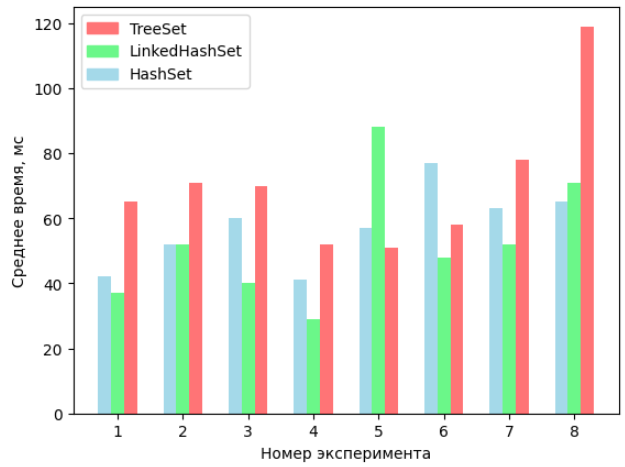
\includegraphics[width=0.8\textwidth]{f_bar}
    \caption{Графическая интерпретация результатов экспериментов при работе с числом файлов исходного кода в 100 единиц}
    \label{fig:f_bar}
\end{figure}

\begin{figure}[H]
    \centering
    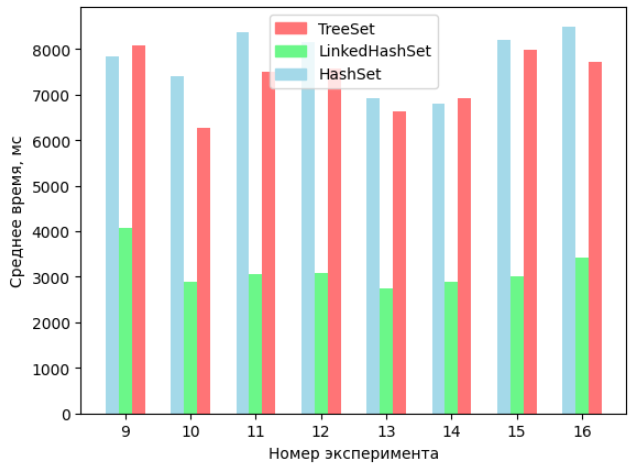
\includegraphics[width=0.8\textwidth]{l_bar}
    \caption{Графическая интерпретация результатов экспериментов при работе с числом файлов исходного кода в 1000 единиц}
    \label{fig:l_bar}
\end{figure}

Результаты экспериментов показывают, что резкое увеличение времени выполнения преобразования графа происходит при увеличении числа файлов исходного кода, а значительное увеличение числа требований к ПО к такому эффекту не приводит.

Наибольшее значение среднего времени составляет 8496~мс, оно достигается при работе с реализацией HashSet. Наименьшее значение среднего времени достигается при работе с LinkedHashSet. При использовании этой реализации коллекции Set наибольшее значение среднего времени составляет 4061~мс, в то время как для TreeSet максимальное значение среднего времени достигает 8083~мс в экспериментах по взаимодействию с файлами исходного кода в количестве 1000 единиц.